%-----------------------------------------------------------------------
%
%   UFRJ  - Universidade Federal do Rio de Janeiro
%   COPPE - Coordenação dos Programas de Pós-graduação em Engenharia
%   PEE   - Programa de Engenharia Elétrica
%
%
%   Projeto EMMA - 
%
%                                                        19/out/15, Rio
%                                                        Estevão F. Ferrão
%----------------------------------------------------------------------
%
%  Compilar usando PDFLaTeX
%
%----------------------------------------------------------------------
\documentclass[12pt,a4paper]{article}
\usepackage{macros/ROSApackages}
\usepackage[brazilian]{babel}

%-----------------------------------------------------------------------
%
%   UFRJ  - Universidade Federal do Rio de Janeiro
%   COPPE - Coordena��o dos Programas de P�s-gradua��o em Engenharia
%   PEE   - Programa de Engenharia El�trica
%
%
%   Projeto ROSA - Rob� para opera��o de stoplogs alagados
%
%   Settings
%                                                         Ramon R. Costa
%                                                         20/mar/14, Rio
%-----------------------------------------------------------------------

%---------------------------------------------------------- COLORS -----
%--------------------------------------------------- Bright colors -----
\definecolor{brightred}     {rgb}{1.00, 0.95, 0.95}
\definecolor{brightgreen}   {rgb}{0.95, 1.00, 0.95}
\definecolor{brightblue}    {rgb}{0.95, 0.95, 1.00}

\definecolor{brightyellow}  {rgb}{1.00, 1.00, 0.95}
\definecolor{brightmagenta} {rgb}{1.00, 0.95, 1.00}
\definecolor{brightcyan}    {rgb}{0.95, 1.00, 1.00}

\definecolor{brightorange}  {rgb}{1.00, 0.95, 0.85}

%----------------------------------------------------- Pale colors -----
\definecolor{palered}     {rgb}{1.00, 0.85, 0.85}
\definecolor{palegreen}   {rgb}{0.85, 1.00, 0.85}
\definecolor{paleblue}    {rgb}{0.85, 0.85, 1.00}

\definecolor{paleyellow}  {rgb}{1.00, 1.00, 0.85}
\definecolor{palemagenta} {rgb}{1.00, 0.85, 1.00}
\definecolor{palecyan}    {rgb}{0.85, 1.00, 1.00}

\definecolor{paleorange}  {rgb}{1.00, 0.85, 0.65}

%---------------------------------------------------- Light colors -----
\definecolor{lightred}     {rgb}{0.95, 0.00, 0.00}
\definecolor{lightgreen}   {rgb}{0.00, 0.95, 0.00}
\definecolor{lightblue}    {rgb}{0.00, 0.00, 0.95}

\definecolor{lightyellow}  {rgb}{0.95, 0.95, 0.00}
\definecolor{lightmagenta} {rgb}{0.95, 0.00, 0.95}
\definecolor{lightcyan}    {rgb}{0.00, 0.95, 0.95}

\definecolor{lightgray}    {rgb}{0.95, 0.95, 0.95}

\definecolor{lightorange}  {rgb}{0.95, 0.63, 0.00}

%--------------------------------------------------- Middle colors -----
\definecolor{midred}     {rgb}{0.85, 0.00, 0.00}
\definecolor{midgreen}   {rgb}{0.00, 0.85, 0.00}
\definecolor{midblue}    {rgb}{0.00, 0.00, 0.85}

\definecolor{midyellow}  {rgb}{0.85, 0.85, 0.00}
\definecolor{midmagenta} {rgb}{0.85, 0.00, 0.85}
\definecolor{midcyan}    {rgb}{0.00, 0.85, 0.85}

\definecolor{midgray}    {rgb}{0.85, 0.85, 0.85}

\definecolor{midorange}  {rgb}{0.85, 0.57, 0.00}

%--------------------------------------------------- Normal colors -----
\definecolor{red}     {rgb}{0.75, 0.00, 0.00}
\definecolor{green}   {rgb}{0.00, 0.75, 0.00}
\definecolor{blue}    {rgb}{0.00, 0.00, 0.75}

\definecolor{yellow}  {rgb}{0.75, 0.75, 0.00}
\definecolor{magenta} {rgb}{0.75, 0.00, 0.75}
\definecolor{cyan}    {rgb}{0.00, 0.75, 0.75}

\definecolor{gray}    {rgb}{0.75, 0.75, 0.75}

\definecolor{orange}  {rgb}{0.75, 0.50, 0.00}

%--------------------------------------------------- Shadow colors -----
\definecolor{shadred}     {rgb}{0.65, 0.00, 0.00}
\definecolor{shadgreen}   {rgb}{0.00, 0.65, 0.00}
\definecolor{shadblue}    {rgb}{0.00, 0.00, 0.65}

\definecolor{shadyellow}  {rgb}{0.65, 0.65, 0.00}
\definecolor{shadmagenta} {rgb}{0.65, 0.00, 0.65}
\definecolor{shadcyan}    {rgb}{0.00, 0.65, 0.65}

\definecolor{shadgray}    {rgb}{0.65, 0.65, 0.65}

\definecolor{shadorange}  {rgb}{0.65, 0.43, 0.00}

%--------------------------------------------------- Darker colors -----
\definecolor{darkred}     {rgb}{0.50, 0.00, 0.00}
\definecolor{darkgreen}   {rgb}{0.00, 0.50, 0.00}
\definecolor{darkblue}    {rgb}{0.00, 0.00, 0.50}

\definecolor{darkyellow}  {rgb}{0.50, 0.50, 0.00}
\definecolor{darkmagenta} {rgb}{0.50, 0.00, 0.50}
\definecolor{darkcyan}    {rgb}{0.00, 0.50, 0.50}

\definecolor{darkgray}    {rgb}{0.50, 0.50, 0.50}

\definecolor{darkorange}  {rgb}{0.50, 0.33, 0.00}

%-------------------------------------------------- Hyperref setup -----
\hypersetup{
  breaklinks   = true,
  colorlinks   = true,
  linkcolor    = darkblue,
  anchorcolor  = darkcyan,
  citecolor    = darkred,
  filecolor    = darkorange,
  menucolor    = darkmagenta,
  urlcolor     = darkgreen,
  pdfhighlight = /I,
  pdfstartview = FitH,
  pdfview      = FitH
}

%---------------------------------------------- DOCUMENT STRUCTURE -----

%------------------------------------------------- Page appearance -----
\setlength{\textheight    }{250mm}
\setlength{\textwidth     }{175mm}
\setlength{\footskip      }{10mm}
\setlength{\footnotesep   }{5mm}
\setlength{\headheight    }{10mm}
\setlength{\headsep       }{5mm}
\setlength{\oddsidemargin }{-6mm}
\setlength{\evensidemargin}{-6mm}
\setlength{\topmargin     }{-15.4mm}
\setlength{\marginparsep  }{0pt}
\setlength{\marginparwidth}{0pt}
\setlength{\parindent     }{5mm}
\setlength{\parskip       }{2.5mm}
\setlength{\topmargin     }{-14mm}
\setlength{\columnsep     }{6mm}

\newcommand{\setbaselinestretch}[1]{\renewcommand{\baselinestretch}{#1}}

\newcommand{\setpagecounter}[1]{\setcounter{page}{#1}}

\setbaselinestretch{1.2}

%------------------------------------------------------- Numbering -----
\setcounter{secnumdepth}{3}  % Subsubsection numbering.
\setcounter{tocdepth}{3}     % Subsubsection index.


%---x---

%-----------------------------------------------------------------------
%
%   UFRJ  - Universidade Federal do Rio de Janeiro
%   COPPE - Coordena��o dos Programas de P�s-gradua��o em Engenharia
%   PEE   - Programa de Engenharia El�trica
%
%
%   Projeto ROSA - Rob� para opera��o de stoplogs alagados
%
%   Macros
%                                                         Ramon R. Costa
%                                                         20/mar/14, Rio
%-----------------------------------------------------------------------

%-------------------------------------------------- Text highlight -----
\newcommand{\texthfg}[1]{\textcolor{blue}{#1}}
\newcommand{\texthbg}[1]{\fcolorbox{lightgray}{lightgray}{#1}}
\newcommand{\HI}[1]{\colorbox{yellow}{\textcolor{black}{#1}}}  %% Highlithed text

\newcommand{\BLU}[1]{\colorbox{white}{\textcolor{blue}{#1}}}

%--------------------------------------------------------- Bullets -----
\renewcommand{\labelitemi}{\texthfg{$\bullet$}}                          % First level.
\renewcommand{\labelitemii}{\texthfg{\tiny$\blacksquare$}}               % Second level.
\renewcommand{\labelitemiii}{\texthfg{\scriptsize$\blacktriangleright$}} % Third level.
\renewcommand{\labelitemiv}{\texthfg{\scriptsize$\bigstar$}}             % Fourth level.

%----------------------------------------------------- Date & time -----
\newcount\m
\newcount\n

\def\twodigits#1{\ifnum #1<10 0\fi \number#1}

\def\hours{\n=\time \divide\n 60
  \m=-\n \multiply\m 60 \advance\m \time
  \twodigits\n:\twodigits\m}

\def\hora{\hours}

\def\data{Rio de Janeiro,\  \number\day\  de \ifcase\month\or
  janeiro\or
  fevereiro\or
  mar\c{c}o\or
  abril\or
  maio\or
  junho\or
  julho\or
  agosto\or
  setembro\or
  outubro\or
  novembro\or
  dezembro\or\fi\  de \number\year
}

%---------------------------------------------------------- Useful -----
\def\pee{Programa de Engenharia El�trica\xspace}
\def\PEE{PROGRAMA DE ENGENHARIA EL�TRICA\xspace}

\def\coppe{Coordena��o dos Programas de P�s--Gradua��o em Engenharia\xspace}
\def\COPPE{COORDENA��O DOS PROGRAMAS DE P�S--GRADUA��O EM ENGENHARIA\xspace}

\def\ct{Centro de Tecnologia\xspace}
\def\CT{CENTRO DE TECNOLOGIA\xspace}

\def\ufrj{Universidade Federal do Rio de Janeiro\xspace}
\def\UFRJ{UNIVERSIDADE FEDERAL DO RIO DE JANEIRO\xspace}

\def\rrc{Ramon Romankevicius Costa\xspace}
\def\RRC{RAMON ROMANKEVICIUS COSTA\xspace}

\def\gscar{Gru\-po de Si\-mu\-la\-��o e Con\-tro\-le em Auto\-ma\-��o e Ro\-b�\-ti\-ca\xspace}
\def\GSCAR{GRUPO DE SIMULA��O E CONTROLE EM AUTOMA��O e ROB�TICA\xspace}

%------------------------------------------------------------ ROSA -----
\def\ROSA{\texthfg{ROSA}}
\def\LROSA{\ROSA\ -- \textit{Stoplog Inspection}}

%\def\ROSA{\BLU{\textsc{ROSA}}\xspace}

%----------------------------------------------------------------------
\newfont{\grande}{cmss10 scaled 1500}
\newfont{\Grande}{cmss10 scaled 2500}
\newfont{\GRANDE}{cmss10 scaled 3500}
\newfont{\enorme}{cmdunh10 scaled 6000}

\newcommand{\block}[2]{
  \def\TXT{~#1~}
  \noindent\TXT \hfill
  \parbox[t]{ \textwidth - \widthof{\TXT} - 2mm}{#2} \\
}

\newcommand{\participantes}[1]{
  \block{\textbf{Participantes}:}{#1}
  \medskip%
}

\newcommand{\pauta}[1]{
  \block{\textbf{Pauta}:}{#1}
  \medskip%
}

\newcommand{\dado}[2]{
  \noindent%
  \makebox[30mm][l]{\sf#1 {\small\dotfill}} :
  \hfill\parbox[t]{140mm}{#2} %\\[2mm]
  \par
  \vspace*{0.30mm}
}

\newcommand{\vu}[2]{ %Utiliza��o: \vu{valor}{unidade}
  \textcolor{darkblue}{#1$\,#2$}\xspace
}

\def\alana{Alana Monteiro\xspace}
\def\antonio{Ant�nio\xspace}
\def\jacoud{Alessandro Jacoud\xspace}
\def\andre{Andr� Figueir�\xspace}
\def\breno{Breno Bellinati de Carvalho\xspace}
\def\elael{Eduardo Elael\xspace}
\def\gabriel{Gabriel Alc�ntara\xspace}
\def\gizele{Gizele Ferreira da Silva\xspace}
\def\julia{J�lia Campana\xspace}
\def\patrick{Patrick Paranhos\xspace}
\def\rafael{Rafael Oliveira\xspace}
\def\ramonC{Ramon Campos\xspace}
\def\ramon{Ramon Romankevicius\xspace}
\def\renan{Renan Freitas\xspace}
\def\sylvain{Sylvain Joyeux\xspace}

\newcommand{\coordenador}{
  \vspace{1.5cm}
  \hspace{7cm}
  \parbox{7cm}{
    \centering
    \rule[0mm]{70mm}{0.1mm} \\
    \rrc \\[3mm]
    Coordenador do Projeto \\
  }
}

\def\assinaturadocoordenador{
  \vspace{10mm}%
  \parbox[t]{70mm}{
    Aprovado por: \\[5mm]
    \centering
    \includegraphics[width=65mm]{../assinatura/assinatura-digital.jpg} \\[-4mm]
    \rule[2mm]{70mm}{0.1mm} \\
    \rrc \\[3mm]
    Coordenador do Projeto \\
  }
}

\newcommand{\footnotecomendereco}{
  \vfill
  \noindent\rule[0mm]{\textwidth}{0.1mm}
  {\scriptsize \sf
  \begin{minipage}{1.5cm}
    Endere�o :
  \end{minipage}
  \begin{minipage}[t]{8.5cm}
    \rrc \\
    COPPE/UFRJ --- \pee \\
    Caixa Postal 68504 --- CEP 21941-972 \\
    Rio de Janeiro, RJ, Brasil
  \end{minipage}
  \hfill
  \begin{minipage}[t]{4cm}
    \begin{tabbing}
      e-mail\ \= : {\tt ramon@coep.ufrj.br} \\
      Lab.    \> : (21) 3938-8604 \\
      Cel.    \> : (21) 98887-9355
    \end{tabbing}
  \end{minipage}
  }
}

\newcommand{\remetente}{
  \vspace{3cm}
  \parbox{15cm}{
    \rrc \\
    COPPE/UFRJ --- \pee \\
    Caixa Postal 68.504 --- CEP 21941-972 \\
    Rio de Janeiro, RJ
  }
}

\newcommand{\fim}{
  \medskip
  \begin{center}
  \rule[1mm]{30mm}{0.14mm}$\diamond$\rule[1mm]{30mm}{0.14mm}
  \end{center}
}

%---x---

%\def\PATH{file:c:/Users/Ramon/My Documents/projetos/2015/Projeto EMMA}
\begin{document}
%-----------------------------------------------------------------------
%
%   UFRJ  - Universidade Federal do Rio de Janeiro
%   COPPE - Coordenação dos Programas de Pós-graduação em Engenharia
%   PEE   - Programa de Engenharia Elétrica
%
%
%   Projeto EMMA - Metodologia para revestimento robótico de turbinas in situ
%
%                                                        19/out/15, Rio
%                                                        Estevão F. Ferrão
%----------------------------------------------------------------------
\pagestyle{fancy}%
\thispagestyle{fancy}%
\renewcommand{\headrulewidth}  {0.4pt}%
\renewcommand{\footrulewidth}  {0.4pt}%
\lhead{\vspace*{-5mm}
\includegraphics[width=30mm]{logo/lead-logo.jpg}}%
\chead{}%
\rhead{}%
\lfoot{}%
\cfoot{}%
\rfoot{\sf [\hours] \quad \today}%
%---------------------------------------------------------------------
\vspace*{20mm}%

{\grande \textcolor{gray}{Financiamento}}

\vspace{-25mm}%
\hspace{50mm}%

\includegraphics[width=50mm]{logo/esbr-logo.png}
\hspace{10mm}%

\includegraphics[width=40mm]{logo/aneel-logo.jpg}

\vspace{35mm}%
{\grande \textcolor{gray}{Execução}}

\vspace{-25mm}%
\hspace{50mm}%

\includegraphics[width=50mm]{logo/gscar-logo.png}
\hspace{10mm}%
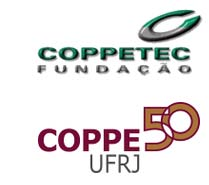
\includegraphics[width=40mm]{logo/coppetec50-logo.jpg}

\vfill%
\begin{center}
  {\GRANDE \raisebox{1.4ex}{} 
\includegraphics[width=80mm]{logo/projeto-EMMA-logo.jpg}} \\[10mm]
  %{\GRANDE \raisebox{1.4ex}{Projeto EMMA} } \\[10mm]
  {\Grande Relatório de Infraestrutura para Testes Finais} \\[25mm]
  {\large \today}
  \vfill%
  %{\Large \today} \\[8mm]
\end{center}

\newpage%
%---------------------------------------------------------------------
\pagestyle{fancy}%
\thispagestyle{fancy}%
\renewcommand{\headrulewidth}  {0.4pt}%
\renewcommand{\footrulewidth}  {0.4pt}%
\lhead{\vspace*{-6mm}
\includegraphics[width=30mm]{logo/lead-logo.jpg}}%
\chead{\vspace*{-6mm}\raisebox{1.7ex}{} 
\includegraphics[width=25mm]{logo/projeto-EMMA-logo.jpg}}%
%\chead{\vspace*{-6mm}\raisebox{1.7ex}{Projeto EMMA}}%
\rhead{\sf\thepage}%
\lfoot{Relatório de Teste Experimental}%
\cfoot{}%
\rfoot{\sf [\hours] \quad \today}%
%---------------------------------------------------------------------

\tableofcontents


\section{Objetivo}
Esse documento tem como objetivo descrever os requisitos mínimos para a
realização dos testes finais para a análise de viabilidade técnica para o
processo de metalização de turbinas \textit{in situ}, como parte final do
projeto EMMA.
Serão descritos os critérios mínimos que os testes devem cobrir e avaliar, assim
como possíveis cenários de teste e o espaço e a infraestrutura
disponíveis e necessários para a realização dos mesmos.

\section{Critérios}
\label{sec::criterios}
\subsection{Cobertura da pá}
Um dos principais requisitos é a capacidade do sistema de posicionar
corretamente o efetuador em toda a superfície da pá utilizando o manipulador
escolhido (Motoman MH12) e o sistema mecânico composto por trilho e base,
garantindo assim uma total cobertura da superfície a ser revestida.
Caso contrário, o processo de metalização não pode ser finalizado
utilizando a solução proposta como único método de
revestimento. Portanto, um dos critérios a ser analisado é o alcance do
manipulador em todos os pontos ou pontos chave previamente selecionados,
obedecendo a restrição de um ângulo de até $30^o$  em
relação à superfície da pá e uma distância entre $0.23m$ e $0.24m$, até a ponta
da pistola de metalização (ou peça representando a mesma).

\subsection{Payload e vibrações}
O processo de metalização utiliza, atualmente, uma pistola com peso aproximado
de $8,5kg$ e necessita de cabeamento até o sistema auxiliar externo.
Para assegurar a qualidade final do revestimento, o processo tem como requisito
uma velocidade constante de $40m/min$ durante o jateamento. 
Portanto, o sistema base e manipulador deverá ser capaz de realizar uma
trajetória pré-estabelecida com um payload de $8,5kg$, na velocidade
especificada, e sofrendo a ação de um empuxo no sentido contrário à ponta do efetuador.

\subsection{Calibração}
A posição relativa entre o manipulador e ao modelo em escala 1:1 da pá deve ser
calculada a partir da nuvem de pontos gerada pelo sensor Faro Focus X330. 
O sistema de calibração também deve ser capaz de identificar e posicionar as pás
do modelo em escala 5:1 em diversas posições do rotor e ângulo de ataque das
pás.

\subsection{Estrutura mecânica}
Deverão ser verificadas a capacidade de montagem da estrutura mecânica, a
robustez do sistema e seu nível de vibrações, quando aplicados as forças
e torques máximos especificados no \textit{datasheet} do manipulador MH12.
A capacidade de posicionamento da base do robô, assim como o pivoteamento entre
o trilho primário e secundário.

\subsection{Shutter}

A capacidade de desvio do fluxo de particulado, antes da queima, deve ser
avaliado, assim como as alterações na pressão no sistema de alimentação.




\section{Espaço disponível}
Atualmente, o único espaço disponível para a realização dos testes é a área
adjacente ao LEAD, dentro do terreno do laboratório.
A utilização desse espaço é restringida por normas e qualquer estrutura a ser
construída no local deve ser aprovada pela arquiteta da UFRJ. 

Foi realizada uma medição do espaço, obedecendo a distância mínima de $1,5m$
da parede e sem obstruir a rampa de acesso da porta de emergência. O espaço
disponível ocupa uma área retangular de $5,40\times3,00m$. O limite de altura
não foi aferido, entretanto a ventilação e a entrada de luz do galpão e prédios
vizinhos devem ser mantidas.




\section{Infraestrutura}
Não existe, no momento, nenhuma infraestrutura no local para as
realização dos testes, sendo necessário a implementação da infraestrutura civil,
elétrica e de suporte para os testes.

Primeiramente, o objetivo principal dos testes consistia em realizar um processo
de pintura automática, simulando o processo de metalização e com forte apelo
visual para o cliente. Entretanto, como será exposto a seguir, a infraestrutura
necessária para o processo é extensa e os paramêtros realmente testados não são
explícitos.

\subsection{Pintura}

Sistema de Pintura: para a utilização de um sistema de pintura é necessária a utilização de sistemas de: 
compressão de ar, purificação de ar, compressão de tinta, isolamento e exaustão.

Compressão de ar: O ar necessário para o sistema deve ser limpo e seco. Para isso é necessário utilizar 
um compressor de diafragma, no qual não existe contato do pistão com o ar a ser comprido ou um filtro de 
óleo. A umidade também afeta o sistema e é necessário a utilização de filtros desumidificadores e condensadores 
de água. Entretanto para o propósito em questão, acredito que apenas um compressor de diafragma seria suficiente, 
pois não há necessidade de uma pintura de qualidade.

Compressão de tinta: As pistolas de tinta podem ser dividas, basicamente, em dois grandes grupos: pistolas a 
gravidade e pistolas automáticas. A primeira classe possui um recipiente onde é
armazenada a tinta e é acoplada à pistola. Essa característica restringe o
movimento do conjunto, forçando que o efetuador fique orientado sempre com o
recipiente na vertical. Essa restrição adicional é desnecessaŕia para o nosso teste e, por isso, desclassifica esse tipo de pistola como um possível dispositivo para a realização do mesmo. A segunda 
categoria utiliza, além da alimentação de ar comprimido, uma alimentação de tinta proveniente de um 
tanque de pressão de tinta.

Outro fator importante é o isolamento da "cabine de pintura" e a correta exaustão do ar do particulado em 
suspensão. A pistola de tinta pulveriza a tinta em direção à peça a ser pintada e parte dessa tinta fica 
em suspensão no ambiente, impregnando as paredes e objetos próximos. A presença humana nesse ambiente requer 
máscaras de respiração e proteção para olhos e roupas, e qualquer equipamento
eletrônico próximo seria danificado, incluindo computadores e o próprio
controlador e manipulador. Sendo assim, é necessário o isolmanento da
área onde será realizada a pintura e proteção do manipulador. Outro ponto a ser
considerado  é a realização de exaustão, filtragem e
descarte corretos da tinta, para que não se danifique nenhuma estrutura
adjacente ao local de testes (LEAD e prédios vizinhos).

A área útil de metalização realizada pela pistola é de 3mm e as pistolas automáticas são para pinturas de grandes 
superfícies, não sendo possível uma cobertura tão precisa. Portanto, o propósito
do teste é prejudicado e a pintura serviria apenas como um indicativo visual,
não representando a real trajetória do efetuador e nem a real cobertura
realizada.

Portanto, não acredito que o investimento de capital, tempo e mão de obra para a construção de uma infraestrutura 
de pintura para o teste de viabilidade técnica para o projeto EMMA 1 justifique os benefícios alcançados por esse 
tipo de procedimento. Outro fator limitante é o espaço ocupado por todos os equipamentos em comparação com o 
espaço disponível no momento, como será apresentado a seguir. Também será apresentado alternativas de testes 
possíveis para ser realizados com o espaço e tempo disponíveis, que consigam avaliar os requisitos mínimos para 
a viabilidade técnica do processo de metalização realizado pelo sistema proposto.  


\subsection{Demanda Elétrica}

O ambiente de testes deve ser dimensionado para suportar uma demanda, além da
consumida pela iluminação e o uso de aproximademente 4 computadores, de 1.5 kVA
relacionada ao controlador DX200 e o manipulador MH12. 
Esses dispositivos operam em sistema trifásico, suportando 240/480/575 V a 50/60. 
O compressor de ar incluíria %TODO potencia do compressor
na demanda total.
Todos os elementos devem ser considerados como de uso
simultâneo. 

A viabilidade de um sistema de resfriação ou ventilação não foi citado pois
depende das características estruturais do projeto. 

\subsection{Base do manipulador MH12}
O manipulador deve possuir uma base padrão instalada no ambiente de testes, para
que seja possível a realização de testes, modificações e reparos na base e
trilho propostos. 
A princípio, não é necessário que a base suporte o robô em
movimento, entrentanto caso haja espaço suficiente, essa possibilidade é
interessante para os testes relacionados apenas ao manipulador sem que haja
influência da base projetada.


\subsection{Movimentação de equipamentos pesados}
O manipulador MH12 deverá ser movimentado constantemente na área de testes e tem
peso de $130kg$, por isso julga-se necessário a implementação de um sistema de
talha e carro trole. O carro trole pode se movimentar em uma viga I pertencente
a própria estrutura de sustentação do ambiente de testes, ou permanente fixada
no mesmo. A estrutura de movimentação deve permitir o transporte entre do
manipulador a partir de sua base até o local de testes de cobertura, para
acoplamento à estrutura mecânica.


\subsection{Bancada de trabalho}
É necessário um espaço para trabalho para pelo menos 1 pessoa.
Primeiramente foi idealizado a utilização da área ocupada pelo controlador DX200
e a construção de uma bancada de apoio. 
Portanto, afim de se poupar espaço, o
controlador ficaria embaixo da bancada e a pessoa trabalhando nos testes usaria
o computador em pé.

 \subsection{Suporte da pá 1:1}
 O suporte da maquete em escala 1:1 da pá deve, idealmente, o giro da pá em
 torno de seu próprio eixo vertical e horizontal. 
 O movimento no eixo vertical possibilita o teste de cobertura em ambos os lados
 da pá, caso contrário é necessário retirar a pá do suporte e realizar o giro.
 É importante ressaltar que dependendo do tamanho do galpão em que o teste seja
 realizado, não será possível a movimentação da pá, sendo necessário a retirada
 da pá de dentro do ambiente para manobra.
 
 \subsection{Fluxo de equipamentos}
 Excluindo-se a instalação da pá discutida na seção \ref{sec::instal_pa}, apenas
o manipulador MH12 e seu controlador representam objetos de dimensões
significativas que deverão passar pela porta de acesso do galpão de testes.
As dimensões do manipulador são e do controlador DX200 são 800(l)   x  650(p) 
x1000(a). 


\subsection{Instalação da Pá}\label{sec::instal_pa}

A fabricação da maquete da pá em escala $1:1$ está prevista para ser iniciada no
laboratório de esculturas da Escola de Belas Artes da UFRJ (EBA)localizado no
prédio da Reitoria, no Fundão.
Esta etapa prevê o recebimento da matéria-prima e o corte das seções que
fomrarão o esqueleto da maquete. 
Foi recomendado que a etapa de montagem e fabricação fosse realizada no nosso
laboratório, evitando assim o transporte que, devido às dimensões do modelo,  só
poderia ser feita por caminhão que, devido a sua fragilidade, traz risco para a
integridade do modelo.
Assim, deve-se prever o espaço para trabalho de fabricação desta na área externa
do LEAD, bem como o armazenamento adequado do produto final, e também, o
armazenamento provisório da maquete, durante a construção do galpão.

\subsection{Fixação da Base}\label{sec::fix_base}

A fixação da base do manipulador pode ser feita de duas maneiras:

\begin{enumerate}
  \item \textbf{Flanges}: Utlizando flanges de fixação com chumbadores (ver
  seção~\ref{sec::chumbadores}), diretamente entre a estrutura da base e o chão.
  Desta forma, limita-se a liberdade de mudança de posicionamento da base, pois 
  cada posição depende de furação do chão e utlização dos chumbadores, criando \textit{spots} de fixação.
  \item \textbf{Placa metálica}: Desta forma, seria instalada uma placa metálica
  de aço com pelo menos $15~mm$ de espessura, fixada com chumbadores. Assim, a
  fixação da base seria por meio das bases magnéticas dimensionadas para
  a solução final. Isto forneceria liberdade de posicionamento para a base do
  robô em qualquer lugar da placa metálica.
\end{enumerate}

 
 \subsection{Chumbadores}\label{sec::chumbadores}
 
 Os chumbadores são elementos de fixação mecânica compostos por parafuso,
 arruela, jaqueta e cone.
 Para fixação da base do robô, seja por qualquer uma
 das soluções propostas na seção~\ref{sec::fix_base} é necessária a utilização 
 de chumbadores devidamente dimensionados, levando-se em consideração os
 esforços  máximos dinâmicos do robô e a geometria da base.
 Assim, uma estimativa inicial prevê a utilização de parafusos com diâmetro de
 rosca de $16~mm$ e profundidade do furo para a jaqueta de, no mínimo $93~mm$.
 
 Logo, deve-se verificar a capacidade do local da instalação para receber os
 chumbadores, sobretudo verificando se os furos não interferem na passagem de
 tubulação de água ou gás.
 
 \subsection{Configuração mínima e espaço disponível}

Atualmente, o único espaço disponível para a realização dos testes é a área
adjacente ao LEAD, dentro do terreno do laboratório.
A utilização desse espaço é restringida por normas e qualquer estrutura a ser
construída no local deve ser aprovada pela arquiteta da UFRJ. 

Foi realizada uma medição do espaço, obedecendo a distância mínima de $1,5m$
da parede e sem obstruir a rampa de acesso da porta de emergência. O espaço
disponível ocupa uma área retangular de $5,40\times3,00m$. O limite de altura
não foi aferido, entretanto a ventilação e a entrada de luz do galpão e prédios
vizinhos devem ser mantidas.

A partir das medidas, foi realizado um esboço de uma configuração
mínima de testes. Como pode ser observado na figura \ref{fig::planta}, a
acomodação dos itens necessários se dá de maneira apertada. A
configuração mínima necessária foi considerada como: uma pá em escala 1:1, uma
seção do trilho primário servindo apenas como ponto de apoio e pivoteamento,
trilho secundário de 2,75m, manipulador MH12 e seu controlador DX200.

\begin{figure}[h!]
\centering
	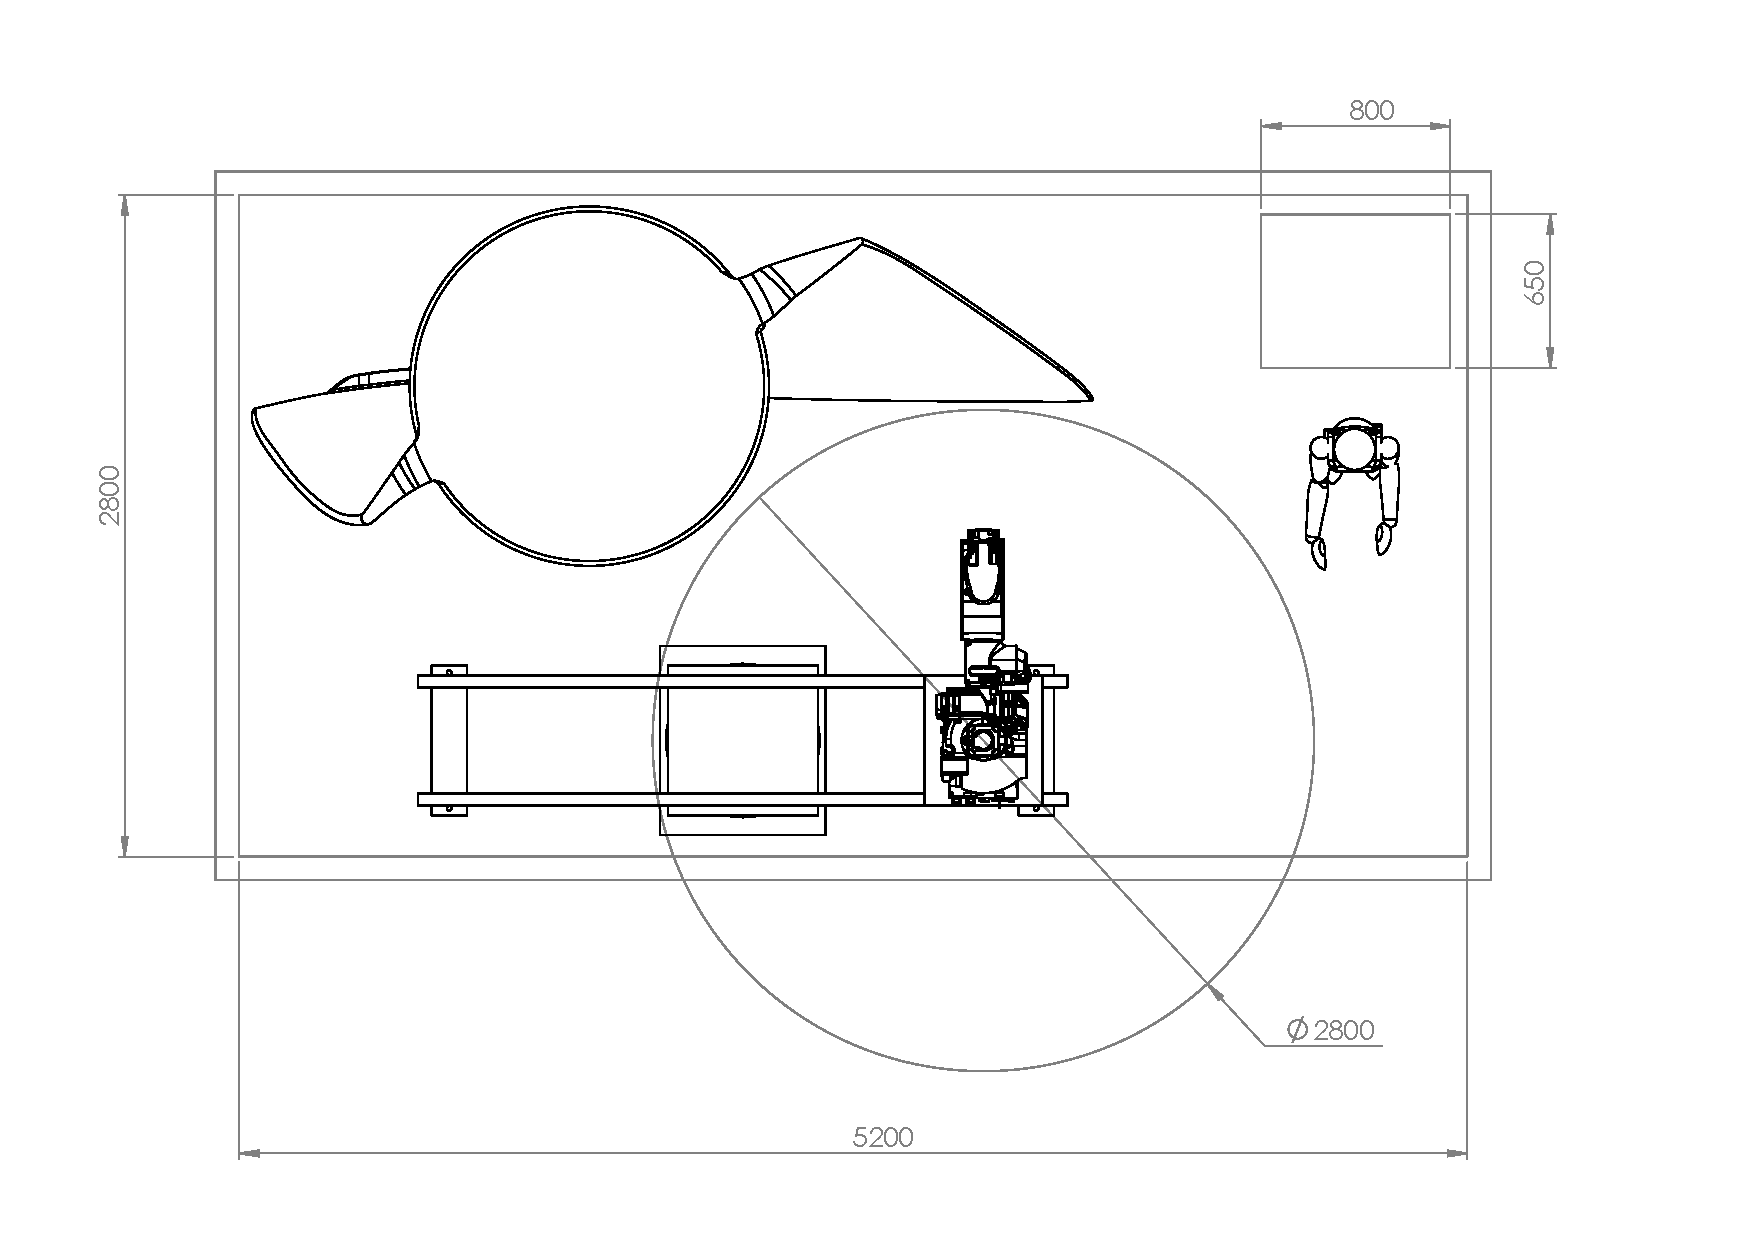
\includegraphics[width=0.9\columnwidth]{figs/espaco/Montagem_Base_LEAD}
	\caption{Espaço disponível e possível disposição dos elementos necessários
	para os testes.}
	\label{fig::planta}
\end{figure}


Pode-se observar que o robô não tem seu espaço de trabalho totalmente livre. As
paredes ficam dentro de seu alcance, representando um perigo estrutural
para o ambiente,  existindo apenas uma posição para a sua base que possibilita
um espaço livre no semi circulo frontal do robô, essa seria a unica área que teríamos para realizar testes 
antes de simular o coating da pá. Esse cenário não é o ideal, uma vez que até o teste final, 
é necessário um espaço para livre movimentação sem risco de colisões.

A viabilidade da utlilização do espaço adjacente ao laboratório em toda a sua
extensão se faz imprescindível para a realização de todos os testes com
segurança. O espaço total disponível mede 10x6.9m e um esboço da possibilidade
de disposição dos equipamentos de testes está exemplificado nas figuras
\ref{fig::planta_grande} e \ref{fig::planta_perspectiva}.

\begin{figure}[h!]
\centering
	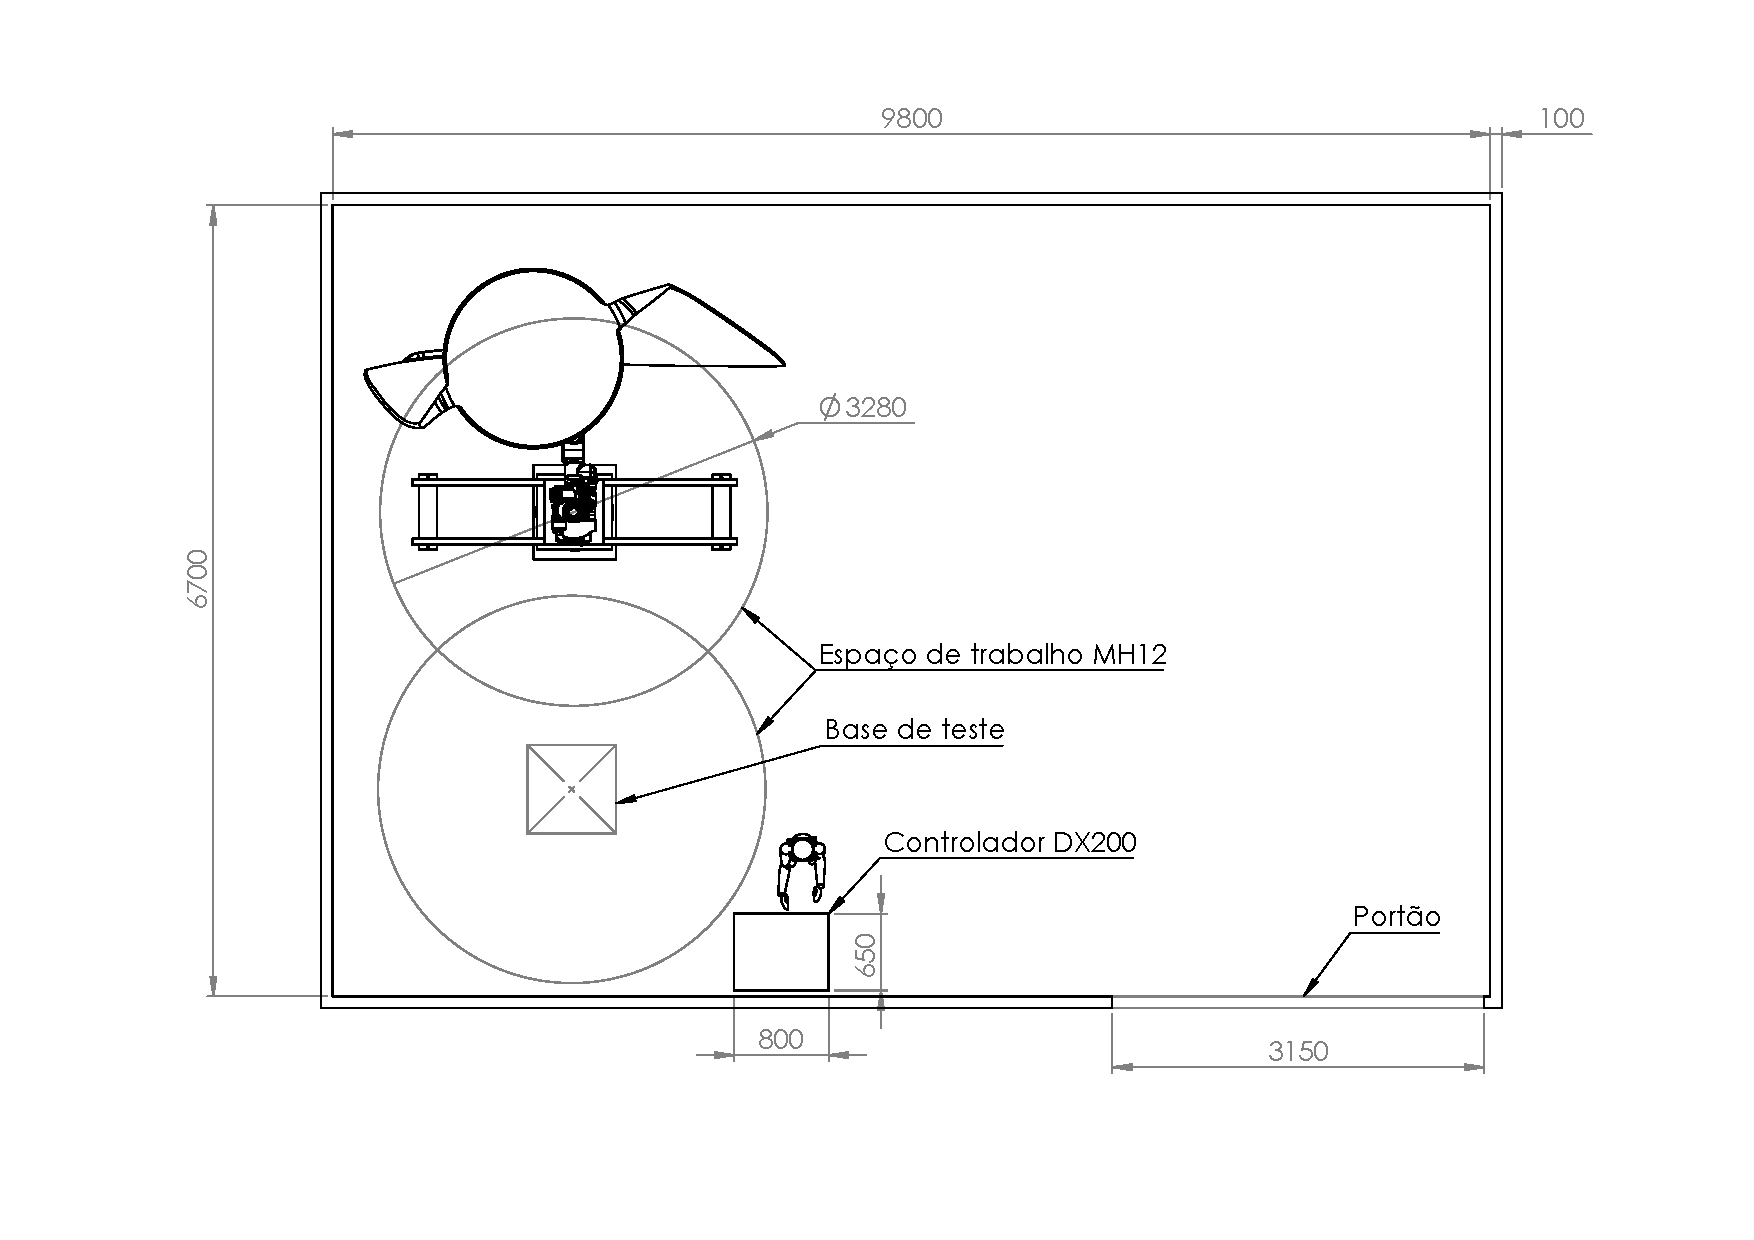
\includegraphics[width=0.9\columnwidth]{figs/espaco/Montagem_Base_LEAD_1}
	\caption{Espaço total disponível e possível disposição dos elementos
	necessários para os testes.}
	\label{fig::planta_grande}
\end{figure}

\begin{figure}[H]
\centering
	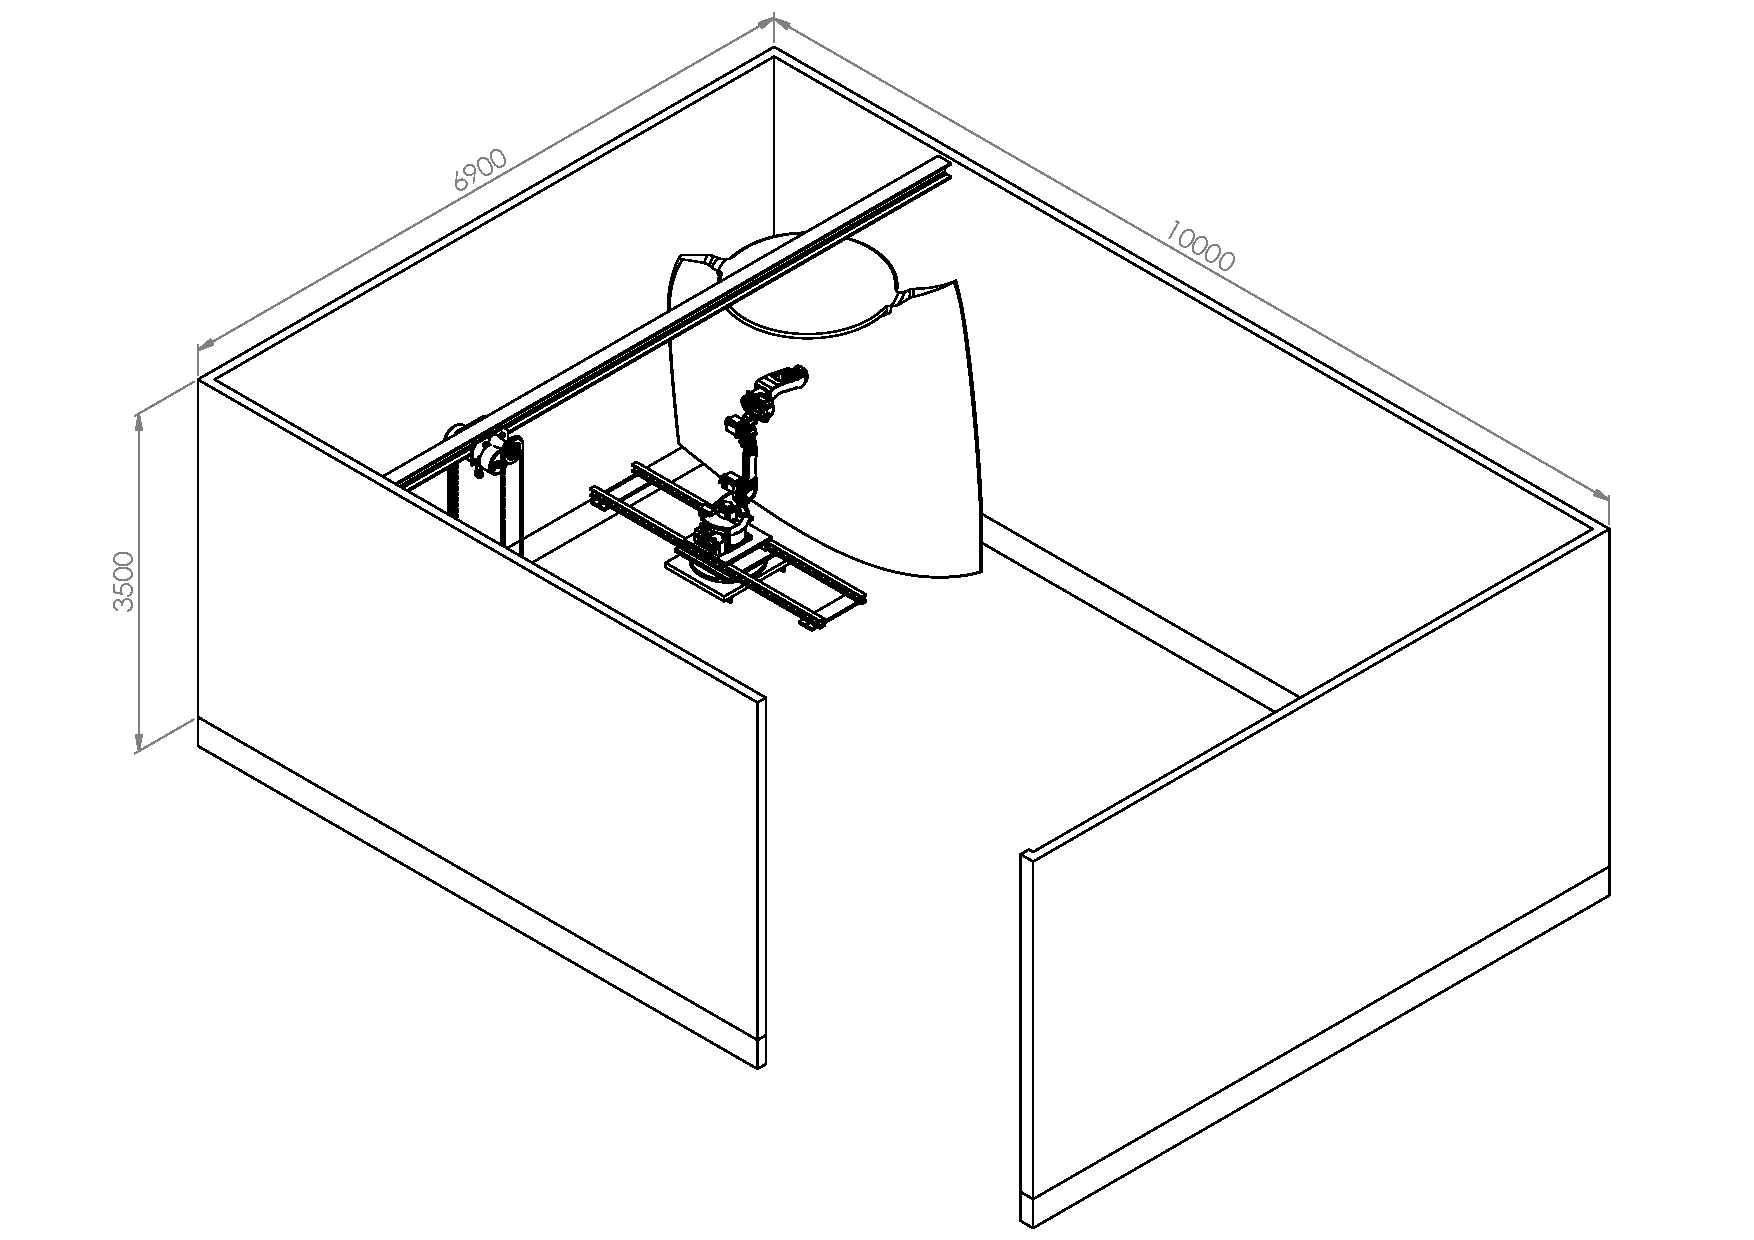
\includegraphics[width=0.9\columnwidth]{figs/espaco/Montagem_Base_LEAD_2}
	\caption{Perspctiva da configuração de testes.}
	\label{fig::planta_perspectiva}
\end{figure}


\section{Testes}
Essa seção apresentará propostas de testes afim de contemplar os critérios
apresentados na seção \ref{sec::criterios}

\subsection{Teste da base}
Devido ao espaço limitado e as configurações
possíveis de fixação, foi analisado que uma possiblidade de testes é avaliar a rigidez estrutural do trilho secundário, 
considerando uma única posição de fixação e sem a necessidade da presença de bases magnéticas. 
O teste contemplaria apenas a rigidez entre o ponto de pivoteamento e o trilho secundário e entre o 
trilho secundário e a base do robô. Assim como a necessidade e possibilidade de uma fixação da base do 
robô diretamente a superfície de apoio.

\subsection{Teste de cobertura da pá}

Visto que uma infraestrura de pintura não apresentou um custo benefício
interessante, outros métodos devem ser propostos.

\begin{itemize}
  \item \textbf{Toque em pontos específicos:} para avaliar a cobertura, seria
  possível um cenário de testes no qual, com o auxílio de um efetuador, o
  manipulador realizaria toques nas partes extremas da pá. A cobertura total
  seria assumida a partir da hipótese que os pontos amostrados são  pontos
  críticos e suficientes.
  \item  \textbf{Pintura com caneta:} afim de garantir o apelo visual para o
  cliente, seria possível realizar um cenário no qual o manipulador realizaria a
  pintura da pá com a ajuda de uma caneta e um efetuador com um sistema de molas
  para garantir uma tolerância em relação à distância da pá. A caneta teria uma
  espessura mais próxima à área útil de metalização da chama, oferecendo uma
  medida mais realista da cobertura da pá se comparada a um sistema de
  pintura.
  \item \textbf{Pintura por \textit{light painting}:} seguindo o mesmo
  raciocínio da pintura com caneta, o robô realizaria uma pintura virtual da pá,
  utilizando um laser e uma câmera para sobrepor toda a trajetória. Esse cenário
  retira a complexidade mecânica e o risco de danificação tanto da pá, quanto da
  caneta, porém adiciona complexidade de implementação e integração do sistema.
\end{itemize}

\subsection{Teste de Calibração}

A partir da infraestrutura proposta, os cenários de testes da calibração seriam
a calibração em escala 1:1 com a pá em posição fixa e o manipulador sendo
movimentado. A calibração pode ser realizada com o sensor sendo posicionado de
maneiras diferentes, com a presença ou não de oclusão. Para a identificação do
cone e diversos posicionamentos da pá, é possível a utlização da maquete 5:1.

\subsection{Payload e vibrações}

Para os testes de payload e vibrações é prosposto a utilização de um lastro
simulando o peso da pistola e um compressor de ar para simuluar o empuxo gerado
pelo processo. Esse compressor pode ser simples e o laboratório já possui um de
dimensões que não atrapalhariam a configuração proposta. É preciso apenas uma
especificação correta das forças geradas pelo processo para o dimensionamento da
vazão de ar necessária e verificação da conformidade do atual compressor.

\section{Shutter}

O estudo do Shutter ainda está em aberto e necessita de mais discussões com a
empresa parceia Rijeza. É possível que os testes desse dispositivos sejam
realizados nas instalações da Rijeza no sul do páis ou na própria usina de
Jirau.



\end{document}
